\chapter{Monte Carlo radiation transport technique theory, code and validation}

\section{Introduction and Background}
The Monte Carlo radiation transport technique is a stochastic method used to model the transport of particles through scattering and absorbing mediums. 

The Monte Carlo method has its roots in Buffon's needle experiment of *date here*. This involved dropping needles over lines spaced L apart and counting how many needles intersect the lines.

%buffons needle fig here?%

The Monte Carlo method is used in various different disciplines. Ranging from use in the financial sector to predict share*more info* to use in statistical analysis to use in modern computer generated images (see \cref{fig:ray-trace}) *ref for all methods*

\begin{figure}
\centering
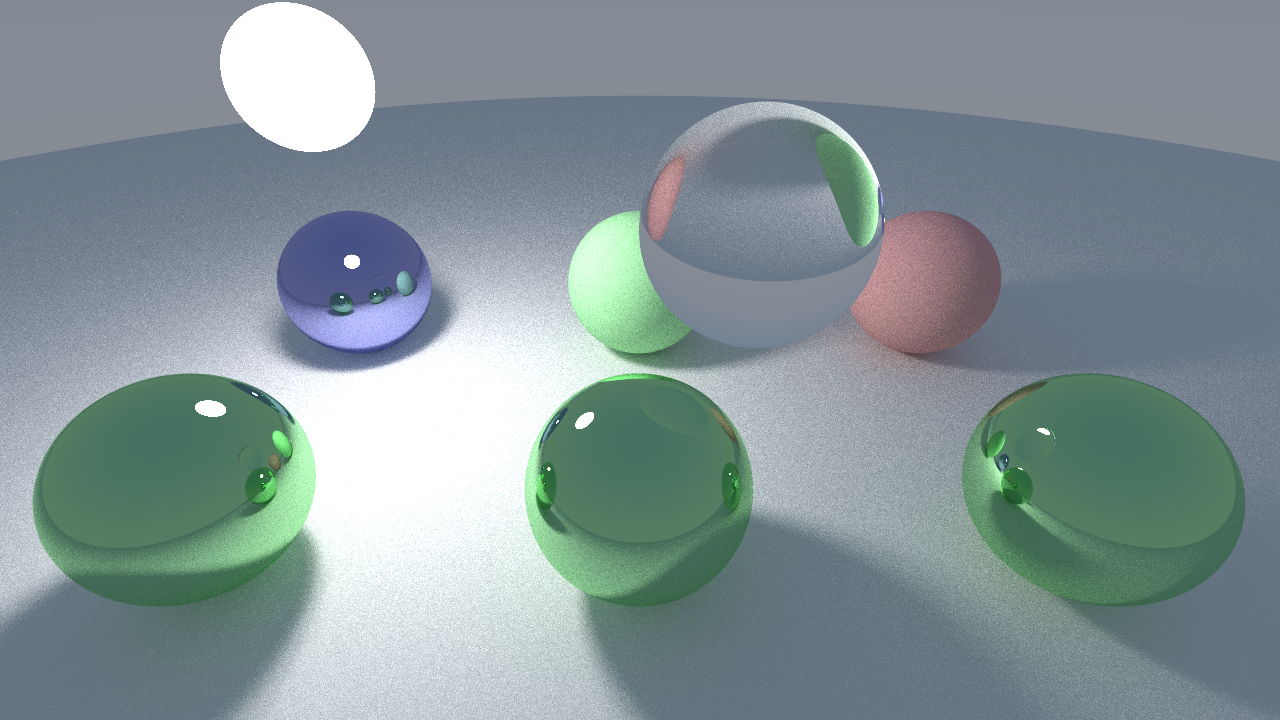
\includegraphics[width=\columnwidth]{./MCRT/images/ray-tracing.png}
\caption{Computer generated imagery using ray-tracing. Code usd to create image available at: github.com/lewisfish/RayTran}
\label{fig:ray-trace}
\end{figure}

The technique that makes up the bulk of this thesis, is the Monte Carlo radiation transport technique. This method was created *correct word?* at the tail end of world war 2 at Los Alamos, for the purpose of calculating neutron diffusion though shielding material *ref*. It has since found amyriad of applications from light transport through dusty clouds, modelling the propagation of proton through tissue for radiotherapy to light transport through tissue.